\documentclass[12pt,a4paper]{report}
\usepackage[latin1]{inputenc}
\usepackage[spanish]{babel}
\usepackage{graphicx}
\usepackage{kpfonts}
\usepackage[left=2cm,right=2cm,top=2cm,bottom=2cm]{geometry}
\author{Bueno Gomez Jorge Heriberto, Briano Garcia Angel Eraclio, Orozco Nevares Josue Natanahel, Alvarez Hernandez Edwin David, Arce Montoya Jonatha,}
\title{Universidad Politecnica de la Zona Metropolitana de Guadalajara\\
Primer avance de proyecto}
\begin{document}
\section{Objetivo general}
Presentar una propuesta para el mejoramiento de la linea de produccion de produccion de envasado, mejorar sustancialmente la eficiencia de una linea de envasado de cerveza de manera exacta, sin que ello conlleve un coste anadido y en un tiempo reducido.
\section{Objetivos especificos:}
Plantear una solucion para el llenado exacto en una linea de produccion
Disenar una linea eficiente con materiales de bajo costo
Estudiar los tiempos de llenado y su produccion 
Determinar los costos de una linea de llenado 
Conocer los datos de costos para la compra de dichos materiales
Verificar la lista de materiales a necesitar
Describir el proceso de llenado que se llevara a cabo
Aumentar la velocidad y eficiencia de los procesos de llenado
Definir un sistema de alarma o errores durante el proceso de llenado
Elaborar la programacion en el lenguaje C++ para la automatizacion de la linea 
Formular un plan de seguridad en caso de error
Automatizar un sistema de llenado
Analizar el proceso de la linea de llenado
Evaluar los tiempos y produccion de la linea 
Proponer una solucion para optimizar el sistema de llenado y taponado de botellas
Mejorar la seguridad de la produccion
Corroborar que todo funcione como deberia
\subsection{Titulo}
Titulo del proyecto
P.I.S.T.O. Siguiendo las siglas de nuestro proyecto serian las siguientes:\\
Portador\\
Inteligente\\
Servicial para\\
Tomadores\\
Organizados\\
\subsection{Delimitacion}
Las delimitaciones del proyecto se consideraron unicamente 3 y son las siguientes:\\
1- El proyecto este programado adecuadamente para su funcionamiento ademas de su correcta construccion.\\
2- Llenar adecuadamente los contenedores de los usuarios que utilicen el P.I.S.T.O. a la medida que el aparato les pueda ofrecer y les otorgue la mayor satisfaccion.\\
3- Economizar en el tema de los recursos al momento de su construccion.
\section{Cual es el problema a resolver?}
Al realizar la investigacion se determina el problema a resolver, el cual es hacer una distribucion casi perfecta de alcohol en bebidas preparadas (alcoholicas).\\
En la recoleccion de informacion y evidencias notamos que el alcohol se desperdicia en pequenas proporciones que al pasar el tiempo en el evento es una perdida de producto y de dinero.\\
Las razones por la que sucede son diversas, descuidos, vasos con demasiado alcohol y por lo tanto lo dejan de beber o lo tiran, caidas, etc.\\
El problema por el cual nos vamos a inclinar a resolver sera:\\
     El suministro adecuado en cada bebida preparada.\\
     El control y proteccion de las bebidas alcoholicas (para evitar accidentes).\\
    Un servicio comodo y sencillo de utilizar.\\
    Rapidez en el servicio.\\
En una posible solucion proponemos una maquina automatizada que se encargue de preparar tu bebida alcoholica.

\section{Objetivos del Proyecto (Como llegar al resultado?)}
En primer lugar, tenemos que plantear un problema para darle una solucion y los integrantes del equipo tenemos un gusto en comun (bebidas alcoholicas). Planteamos una maquina de llenado de alcohol automatizada para poner en practica nuestros nuevos conocimientos que estamos desarrollando en clase.
Surgiendo la idea tenemos que investigar los materiales que serán requeridos y hacer una cotizacion para poder empezar con el ahorro de fondos.
Una vez consultado los materiales necesarios procederemos a aplicar nuestros conocimientos tecnicos de electronica y programacion para estructurar un diseno funcional y facil de utilizar, así como establecer un sistema confiable con la menor probabilidad de errores.
Habiendo terminado con el diseno procederemos a empezar el proceso de ensamblado, en este punto empezaremos un sistema de prueba y error para mejorar fallas que nos puedan salir en el proceso, de esta forma podremos optimizar nuestra maquina automatizada.
Al concluir con el ensamblado solo nos resta mejorar detalles y pequenos errores que puedan salir en un uso cotidiano que para ello lo tendremos a prueba en reuniones del equipo haciendo uso de nuestra maquina automatizada.

\section{Esquema matriz}

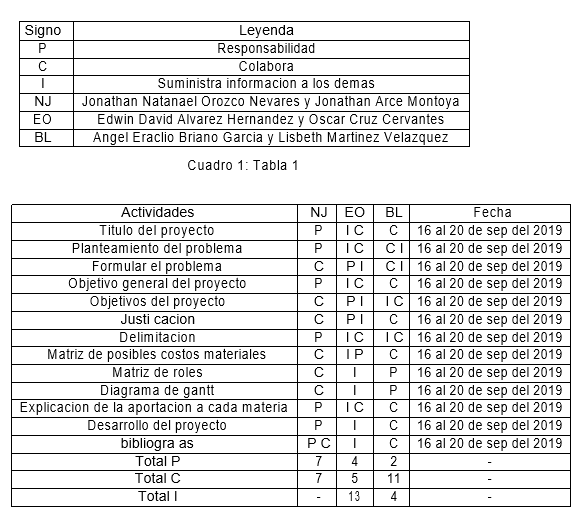
\includegraphics[scale=1]{Esquema de matriz.png} 

\section{Costos}

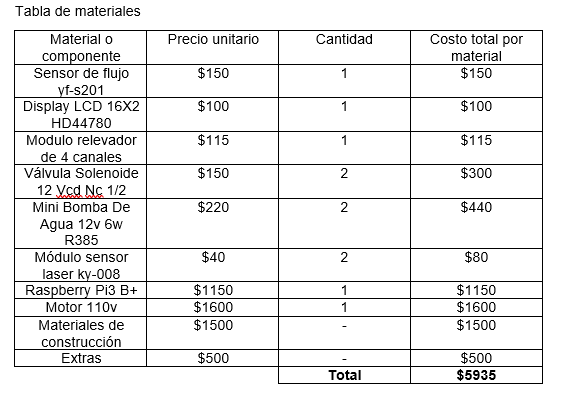
\includegraphics[scale=1]{Costos.png} 

\section{Diagrama}

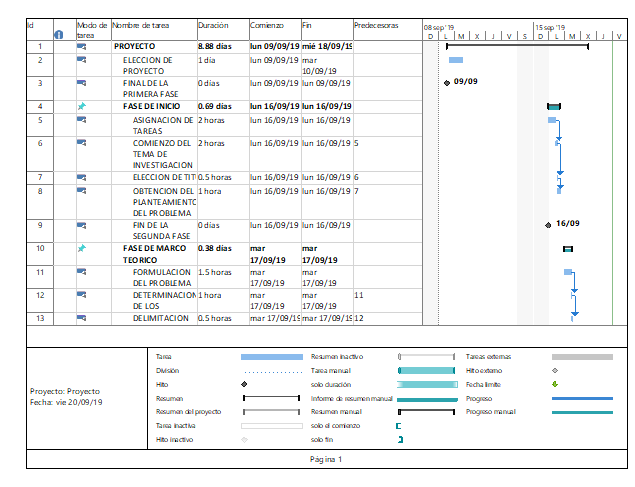
\includegraphics[scale=1]{Diagrama.png} 
\section{Materias relacionadas}
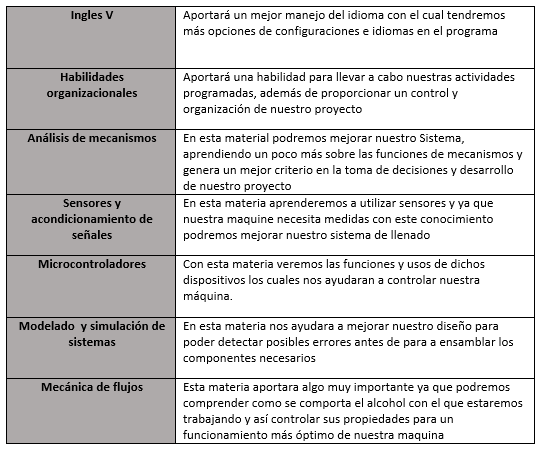
\includegraphics[scale=1]{Materias.png} \\
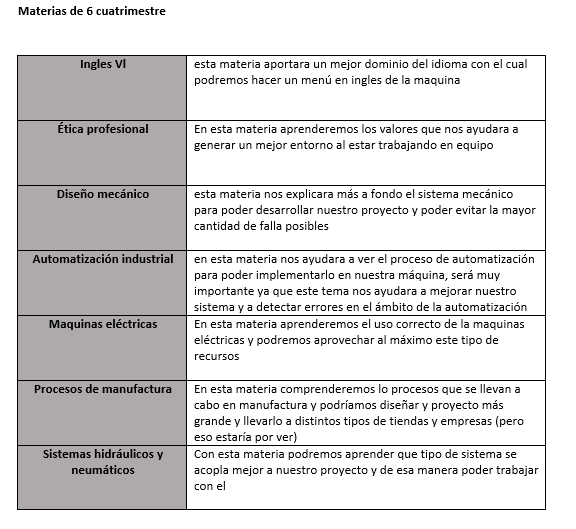
\includegraphics[scale=1]{Materias 1.png} 
\end{document}